\section*{Chemnitzer Linuxtage 2013}
\hypertarget{chemnitz}{}
\label{chemnitz}
\NewsAuthor{Horst JENS}
%\begin{wrapfigure}{r}{2.0cm}
%
\includegraphics[width=2cm]{chemnitz/horst2011mitdoppeltux.jpg}    
%\end{wrapfigure}
\textbf{\textit{Horst JENS} [1] berichtet von den Chemnitzer Linuxtagen 2013 [2], dem erfreulichen Zusammentreffen mit leibhaftigen Open-Source Programmierern, einem Vortrag von \href{http://wiki.skolelinux.de/KurtGramlich/Biografie}{\textit{Kurt Gramlich}} [3] zum Thema \href{http://goo.gl/EoIDpy}{\textit{Linux in Schulen}} [4] und dem \href{http://osdomotics.com}{\textit{OSDomotics}}  [5] Messestand zum Thema \textit{Smart Home}}

\subsection*{Ein Reisebericht}

Der jährliche stattfindende \href{http://chemnitzer.linux-tage.de/2013/}{\textit{Chemnitzer Linuxtag}} [2] vereinigt alles was in der deutschsprachigen Open Source Welt Rang und Namen hat. Ein Wochenende  lang stellen über 400 Aussteller Ihre Open Source Projekte bzw. Firmen vor, es gibt Vorträge und Workshops, Dr.Tux hilft bei Computerproblemen, Kinder basteln mit dem Raspberry Pi und löten Roboter; für den reibungslosen Ablauf sorgt ein Heer engagierter Freiwilliger HelferInnen.

\begin{center}
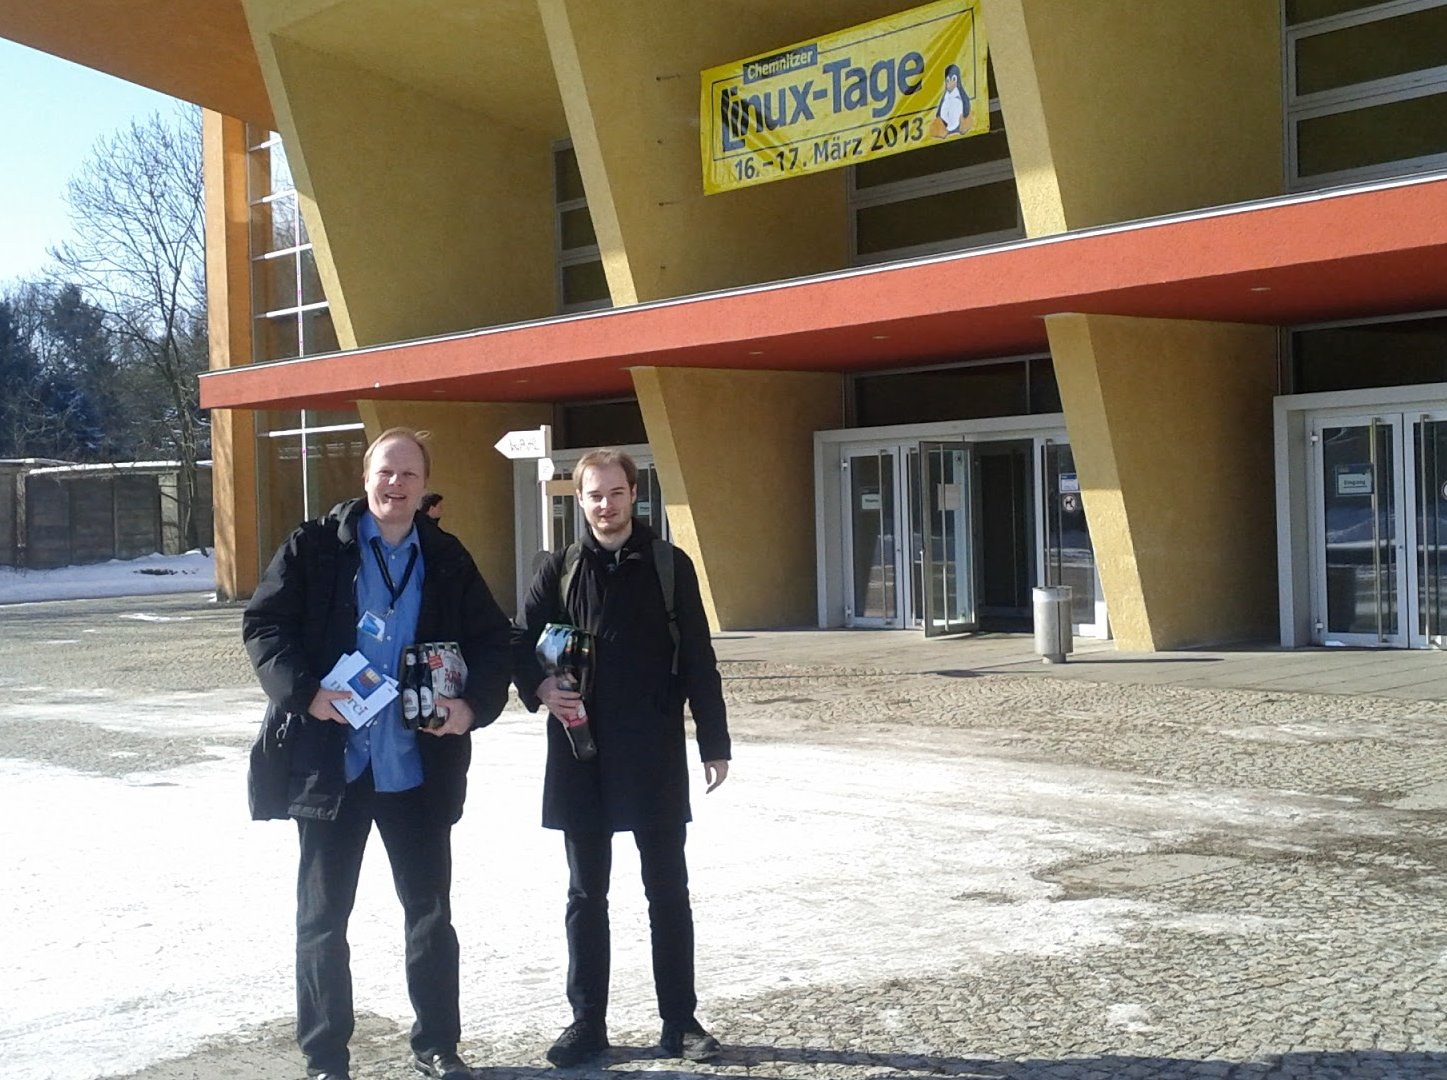
\includegraphics[width=\linewidth]{chemnitz/chemnitz_eroeffnung.jpg}
\footnotesize{Horst JENS und Florian Schweikert. Bildrechte: [1], cc-by-sa}
\end{center}

Für mich war es \href{http://spielend-programmieren.at/de:sonstiges:alter_blog:2009:0318_chemnitzer_linux-tage_2009}{\textit{nach 2009 [6]}} der zweite Besuch auf einem Chemnitzer Linuxtag, dementsprechend erwartungsvoll fuhr ich hin. Meine Reisegruppe bestand aus acht Leuten vom Verein \href{http://osdomotics.com}{\textit{\textbf{OSDomotics} [5]}}. Nach einer langen Zugfahrt (Wien - Nürnberg - Chemnitz) und Ankunft in einem Wolkenkratzer-Hotel (W-Lan im Zimmer nur gegen Aufpreis) machten wir uns auf den Weg zum Gelände der technischen Universität wo der Chemnitzer Linuxtag (\textbf{Hashtag} \#CLT2013) jährlich statt findet.

Der Freitag Abend ist für das Aufbauen und Verkabeln des Messestandes vorgesehen - für das Publikum öffnet sich die Messe erst am Samstag Früh. Die erste schöne Überraschung erlebten wir gleich nach der Ankunft: Es gab erfreulich wenig zu tun, die Organisatoren hatten ganze Arbeit geleistet: Das Messestandplakat war schon ausgedruckt und aufgeklebt, der Tisch war schon hergerichtet (inkl. Stromkabeln und Sesseln), Ausstellerausweise mit Essensgutscheinen und Workshop / Vortragsverzeichnis lagen schon bereit, und das W-Lan funktionierte einwandfrei. 

Bei andere Messen (nicht nur Linuxtage, sondern auch kommerziellen Messen) ist eine so gute Organisation keineswegs selbstverständlich.


\subsection*{Bier und Schokolade}

\begin{center}
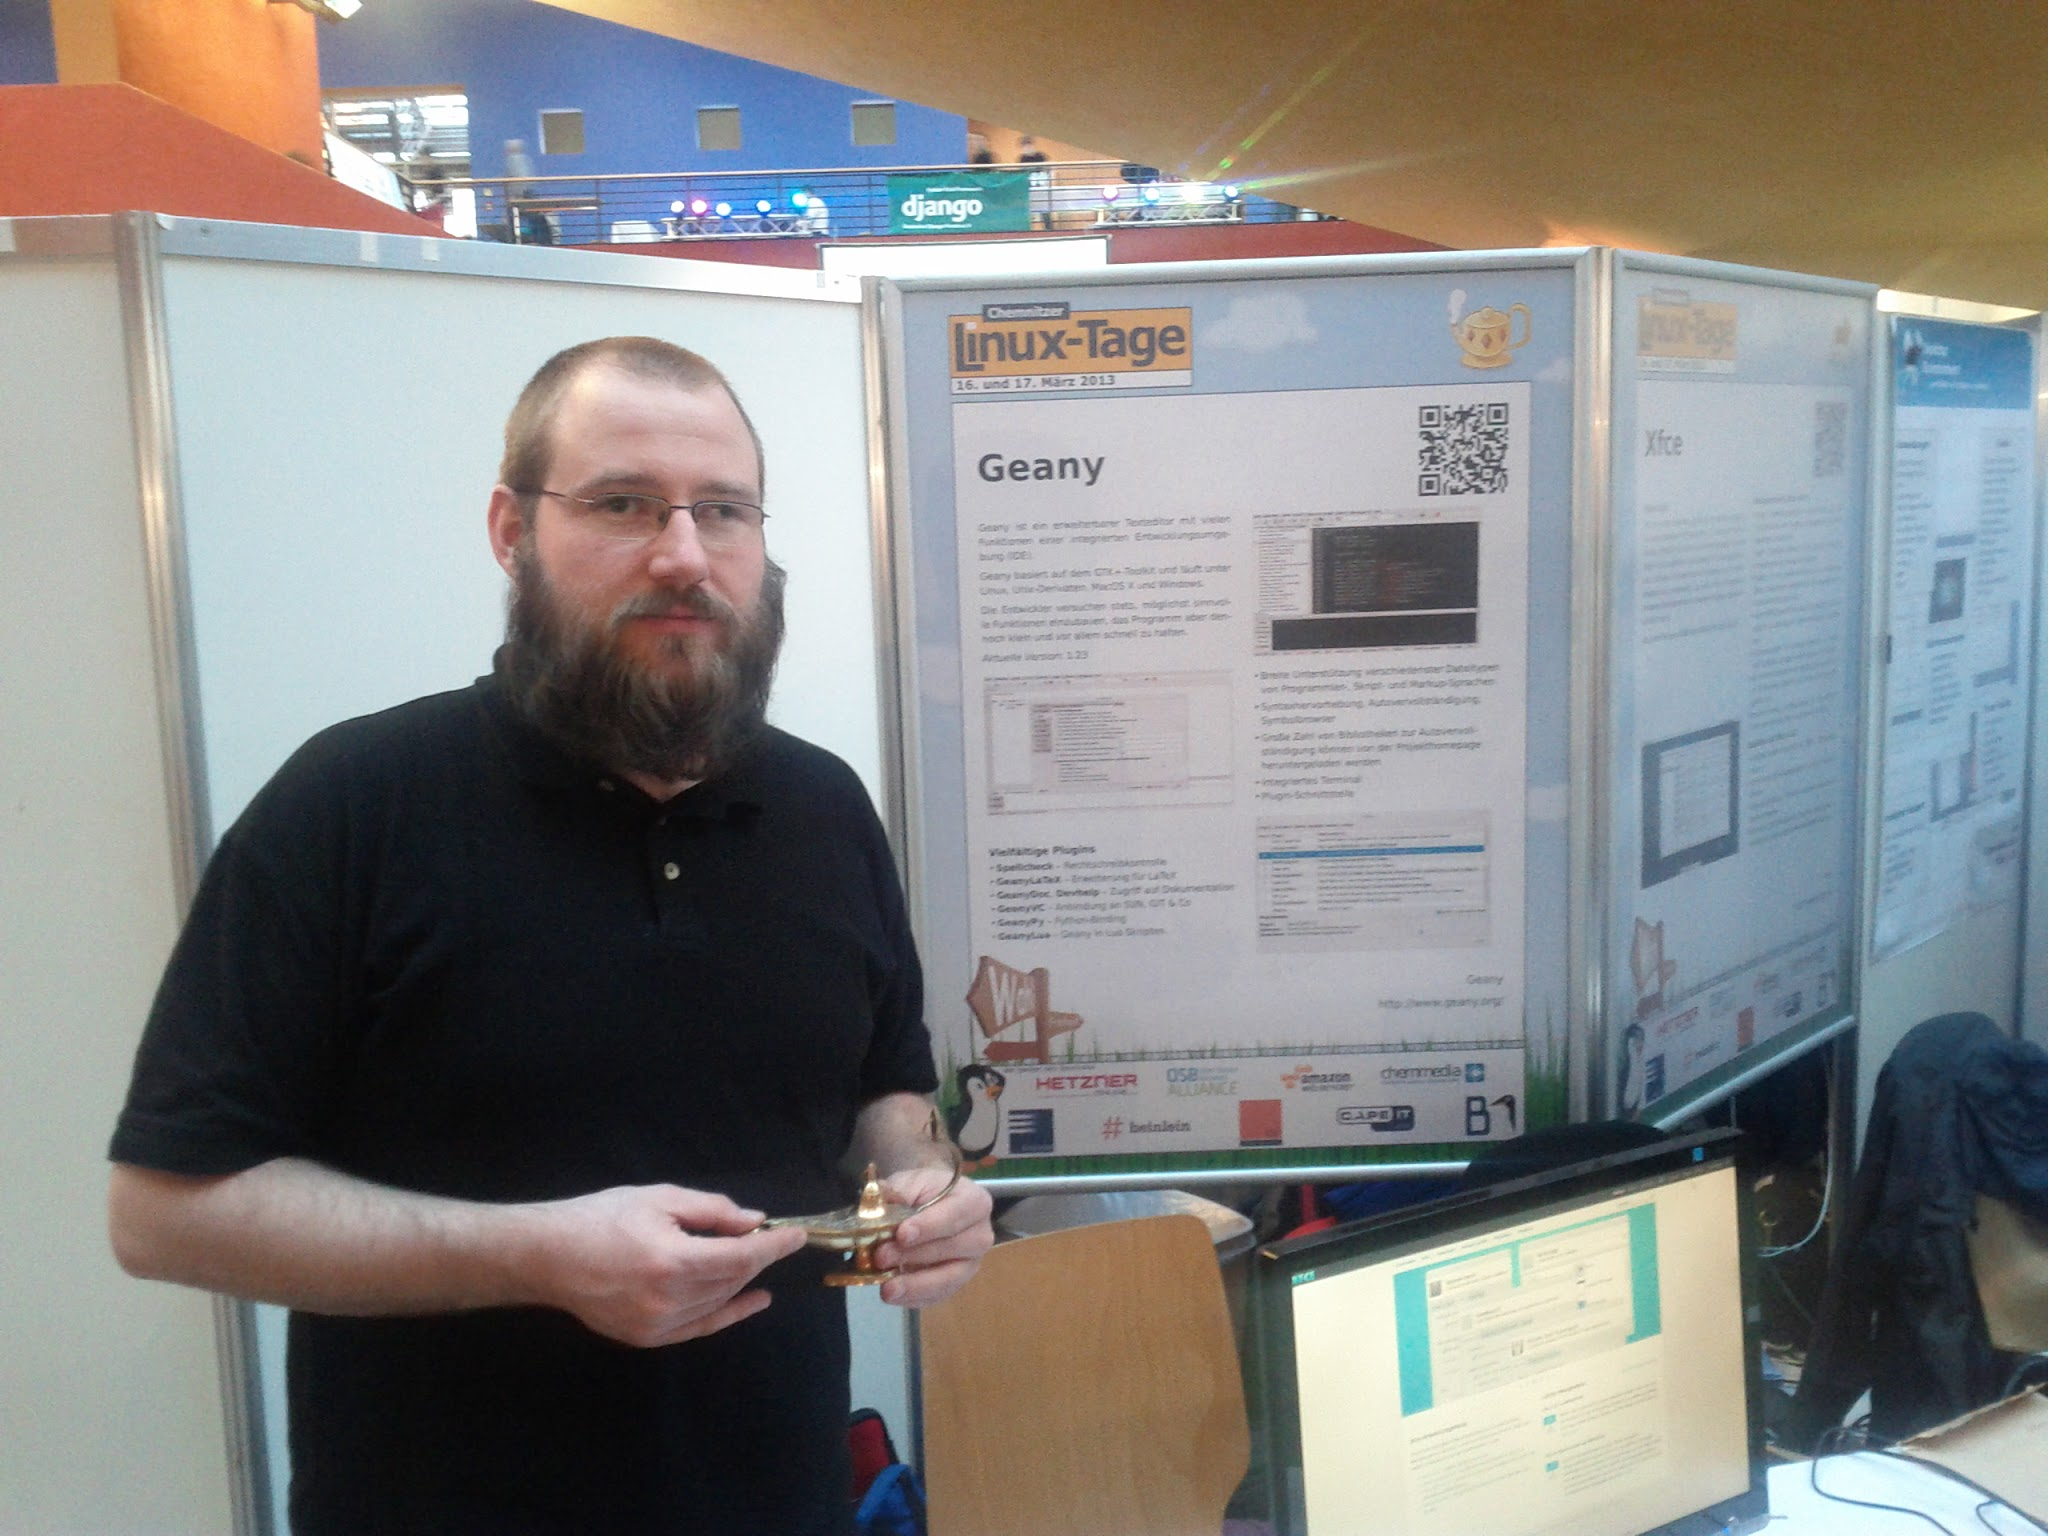
\includegraphics[width=\linewidth]{chemnitz/chemnitz_geany1.jpg}
\footnotesize{Geany Entwickler bekommt Schokolade. Bildrechte: [1], cc-by-sa}
\end{center}

Nachdem Aufbau unserer Messeattraktion (ein Puppenhaus mit \textbf{6LoWPAN} Funksensoren und Lichtern) schlenderte ich mit \textit{Florian Schweikert [7]} (bekannt vom \textit{Biertaucher-Podcast [8]}) durch die Messehalle um die anderen Standplakate anzuschauen. Zu unserer großen Freude entdeckten wir vom freien Programmiereditor \href{http://geany.org/}{\textbf{Geany}} und vom Python Framework \href{https://www.djangoproject.com/}{\textbf{Django}} eigene Messestände. Spontan beschlossen wir am Samstag mit Bier und Schokolade bei den Projektbetreibern vorbei zu schauen.

Am Samstag (nach einem Spaziergang durch das eher menschenleere Chemnitz) kam unsere Geschenkaktion sehr gut an. Geany wird von einem über die ganze Welt verstreuten Team von  Open Source Programmierern (unentgeltlich) entwickelt, und die beiden anwesenden Entwickler aus Deutschland waren sichtlich erfreut über ein Stück handfeste Dankbarkeit. Die Geany Homepage hat mittlerweile zusätzlich zum \href{https://www.paypal.com/cgi-bin/webscr?cmd=_s-xclick&hosted_button_id=8049199&lc=GB}{\textit{PayPal Link}} auch einen  \href{http://flattr.com/thing/1151425/Geany}{\textbf{Flattr} Spendenbutton}. 

\begin{center}
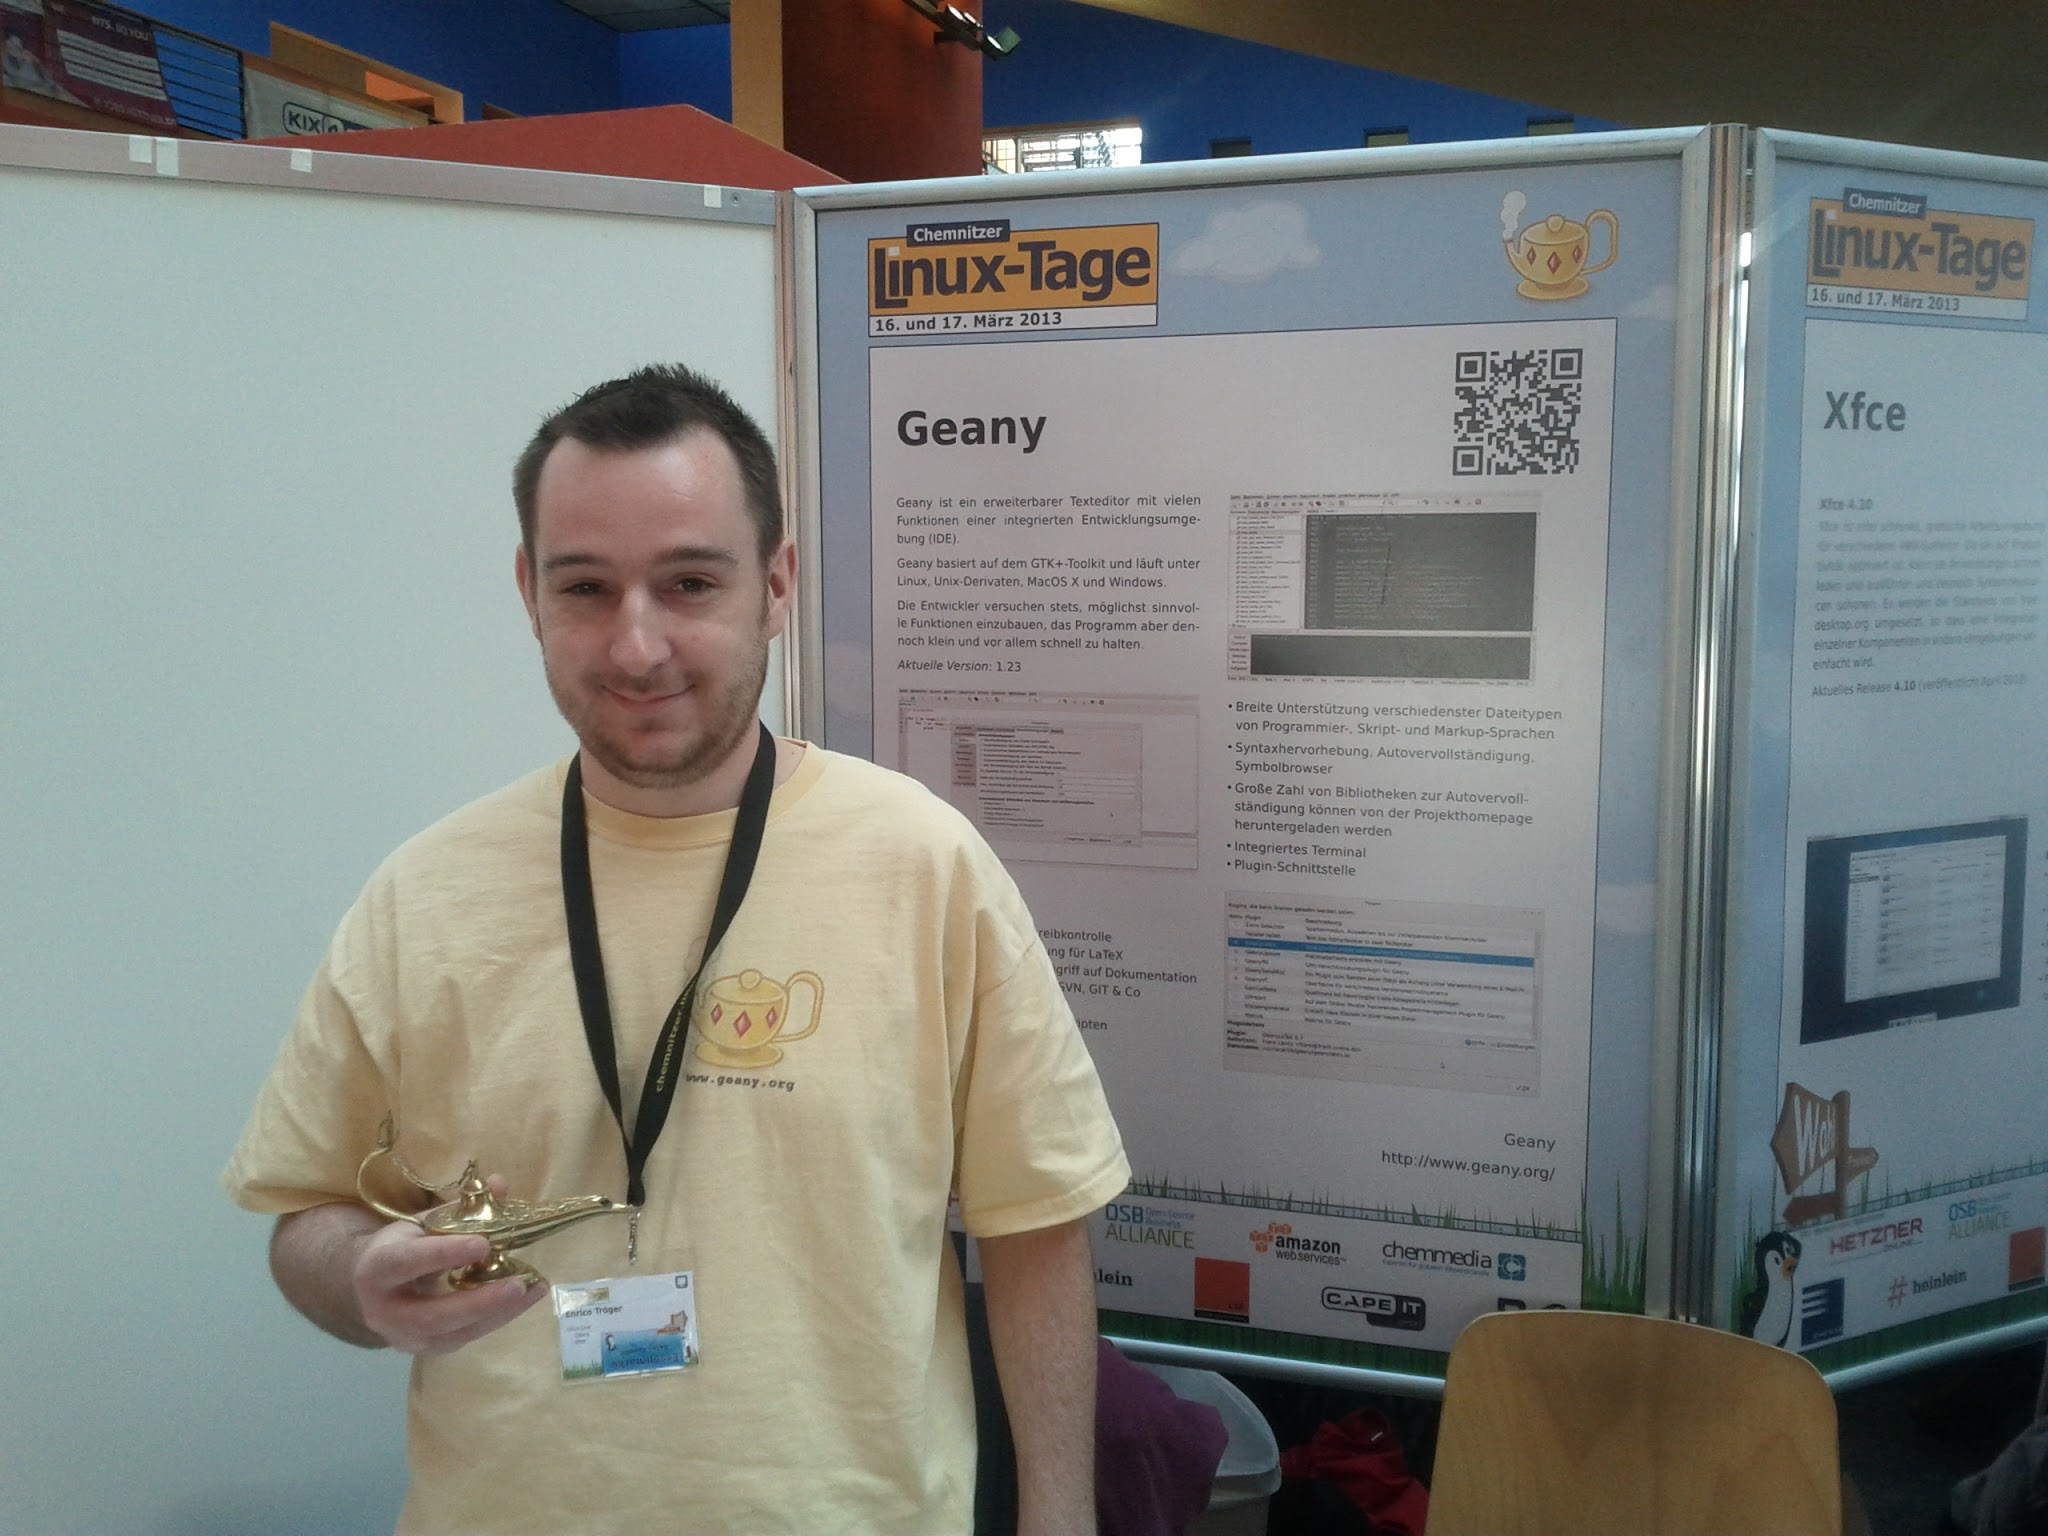
\includegraphics[width=\linewidth]{chemnitz/chemnitz_geany2.jpg}
\footnotesize{Geany der Flaschengeist. Bildrechte: [1], cc-by-sa}
\end{center}

Ebenso freute sich der anwesende Django Entwickler, der stellvertretend für die in der \href{https://www.djangoproject.com/foundation/}{\textit{Django-Foundation}} organisierten  Programmierer das Bier annahm und versprach es so gerecht wie möglich zu verteilen. Uns machte das Schenken ebenfalls große Freude, vielleicht entsteht eine kleine nette Tradition daraus.

Da der OSDomotics Messestand mit acht Leuten sehr gut bemannt war hatte ich ein wenig Zeit mir am Samstag die anderen Messestände anzusehen und sogar zwei Vorträge zu besuchen. Weil ich nach Möglichkeit mit jedem Messestandpersonal (eigentlich gab es keine uninteressanten Messestände) kurz plaudern wollte verging der Samstag wie im Flug. 

Am Abend eröffnete eine Trommlertruppe das große Festbuffet, spät am Abend fuhr die OSDomotics Gruppe gut gelaunt, aber müde zurück ins Hotel.

\begin{center}
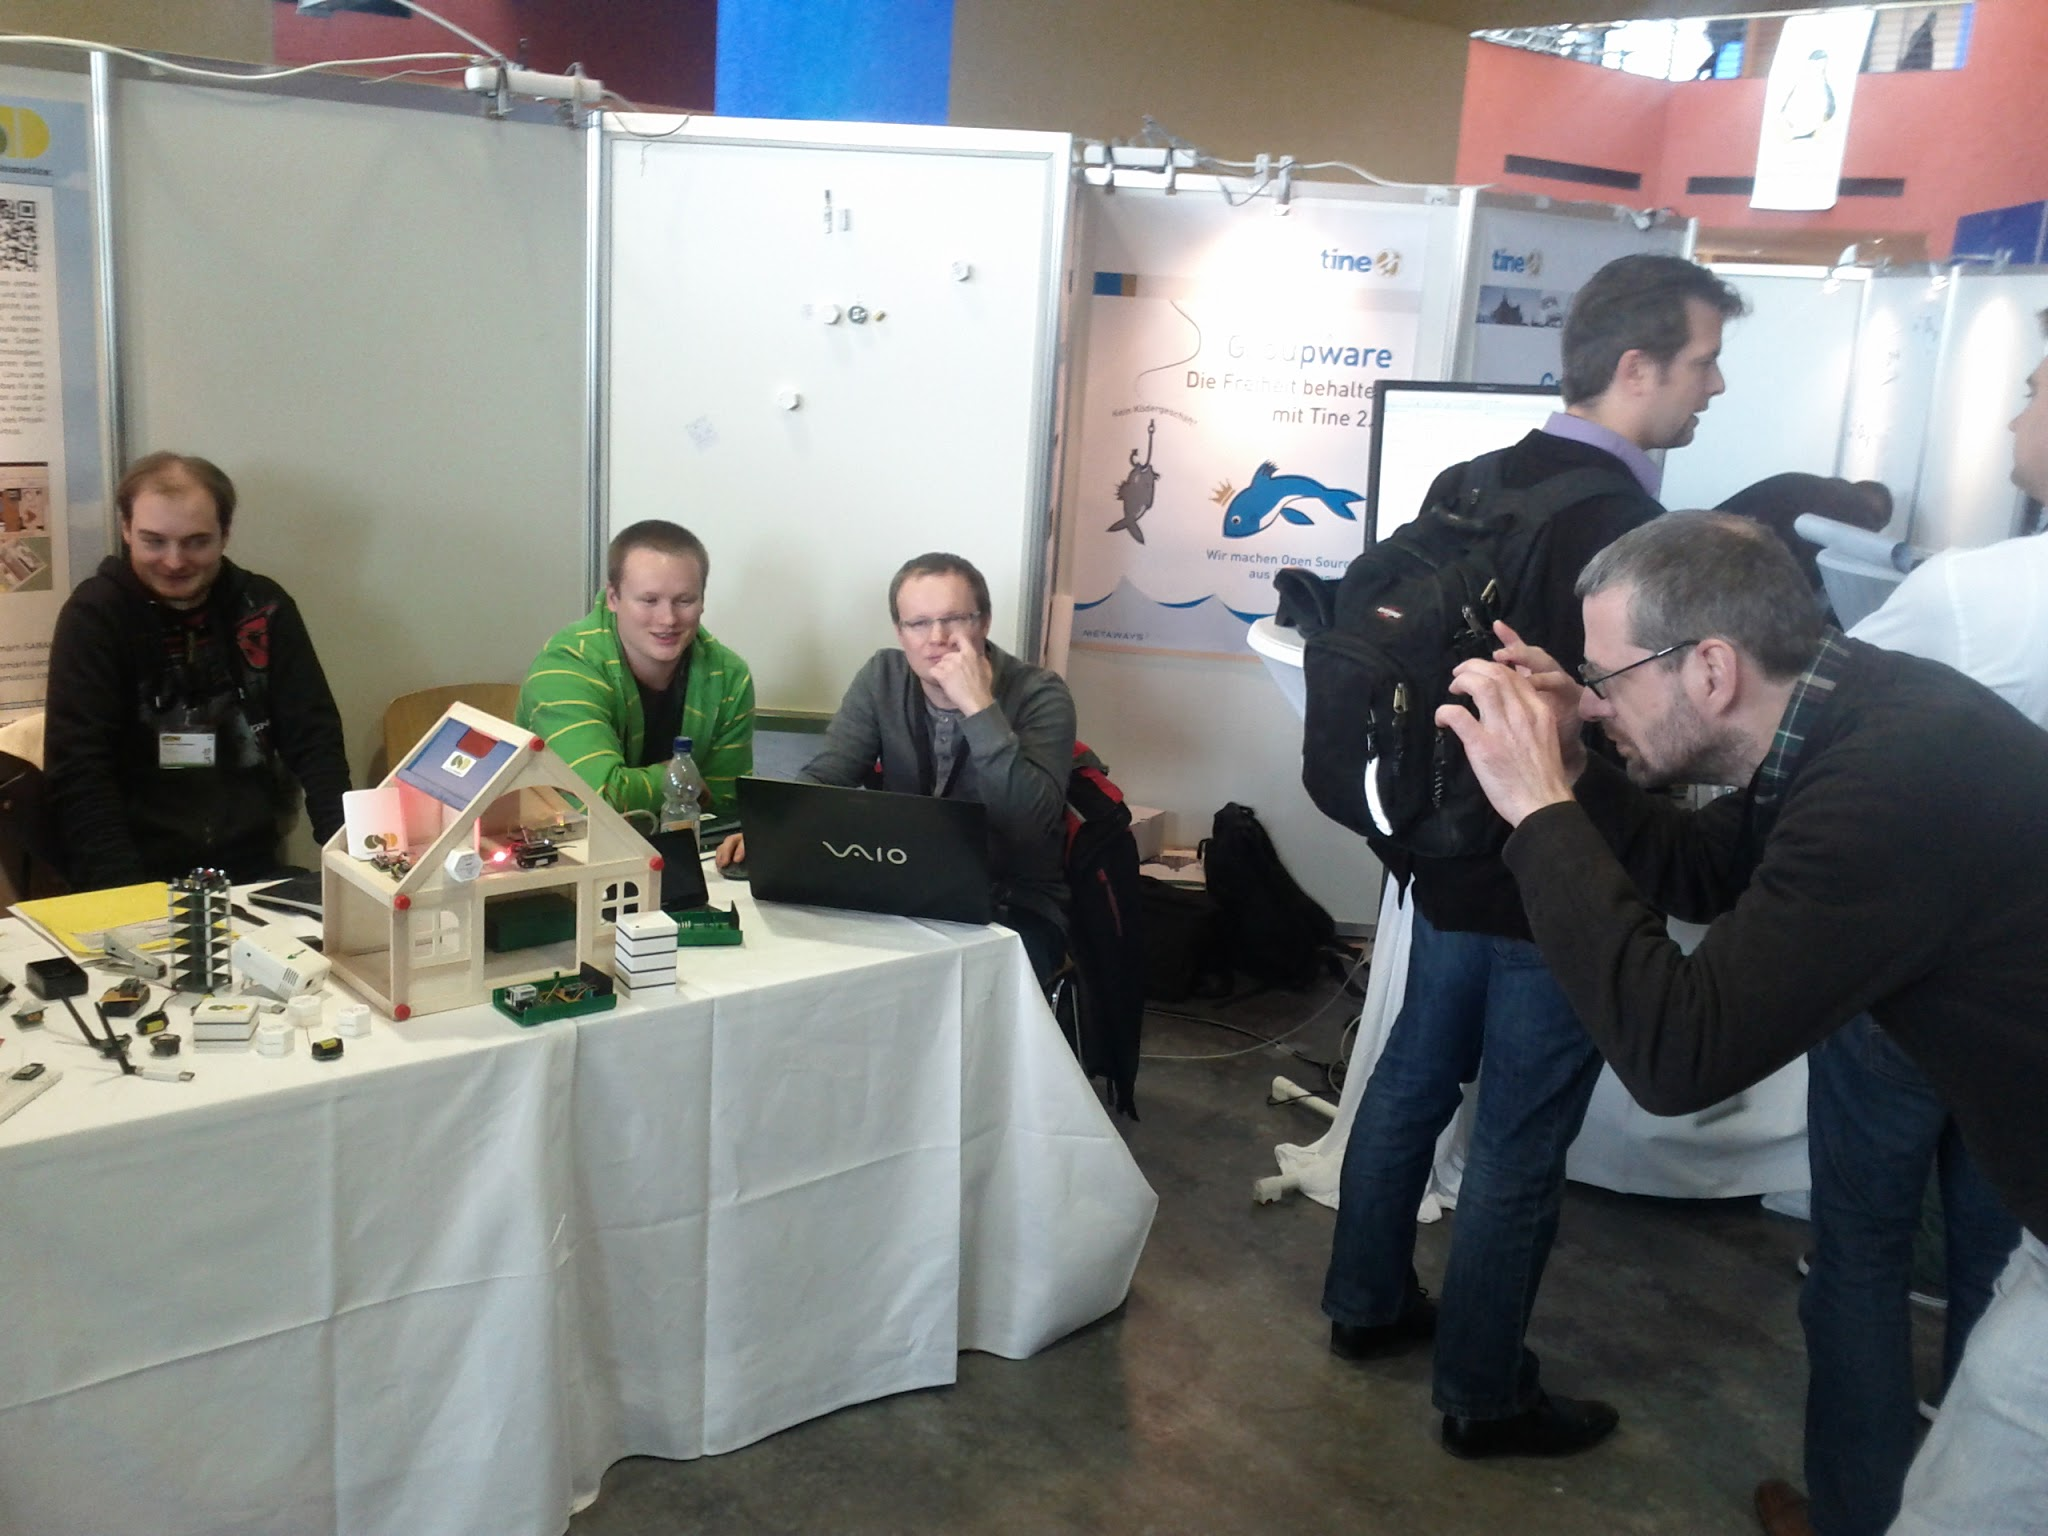
\includegraphics[width=\linewidth]{chemnitz/chemnitz_puppenhaus.jpg}
\footnotesize{Unser Messestand. Rechts im Bild mit Fotoappart: Harald Pichler, Verein OSDomotics. Bildrechte: [1],  cc-by-sa}
\end{center}

\subsection*{Kleinunternehmen}

Am Sonntag war deutlich weniger Publikumsandrang als am Samstag, der OsDomotics Messestand war trotzdem immer gut besucht. Erst um 16:00 gelang es mir ein Foto vom Messestand ohne Besucher davor zu machen. Nur zwei Vorträge konnte ich vollständig besuchen: Einen Vortrag von zwei selbständigen Computer / Open Source Beratern welche dazu aufriefen kleine Unternehmen zu betreuen anstatt sich auf große Unternehmen zu konzentrieren. Die Zahlen für Deutschland, Österreich und Schweiz ähneln sich: 

Circa 80 Prozent aller Unternehmen sind sogenannte \textit{Kleinunternehmen} mit weniger als 10 Mitarbeitern. (Die Definition \textit{Kleinunternehmen} ist von Land zu Land unterschiedlich). Und während diese Masse kleiner Unternehmen nur einen geringen Anteil am Gesamtumsatz hat -siehe \textbf{Paretoprinzip}-, so stellen sie doch eine große Masse an potentiellen Kunden. Meist mit knappem Budget und eigenwilligen Prioritäten (\textit{Das Ding soll funktionieren sonst schreib' ich die Rechnungen mit der Schreibmaschine}). 

Wie die beiden Vortragenden in einer Art Doppelconference darlegten haben kleine Unternehmen einen Vorteil den es bei großen Unternehmen nicht gibt: Aus erfolgreicher Arbeit bei kleinen Unternehmen entstehen oft persönliche Freundschaften.

\begin{center}
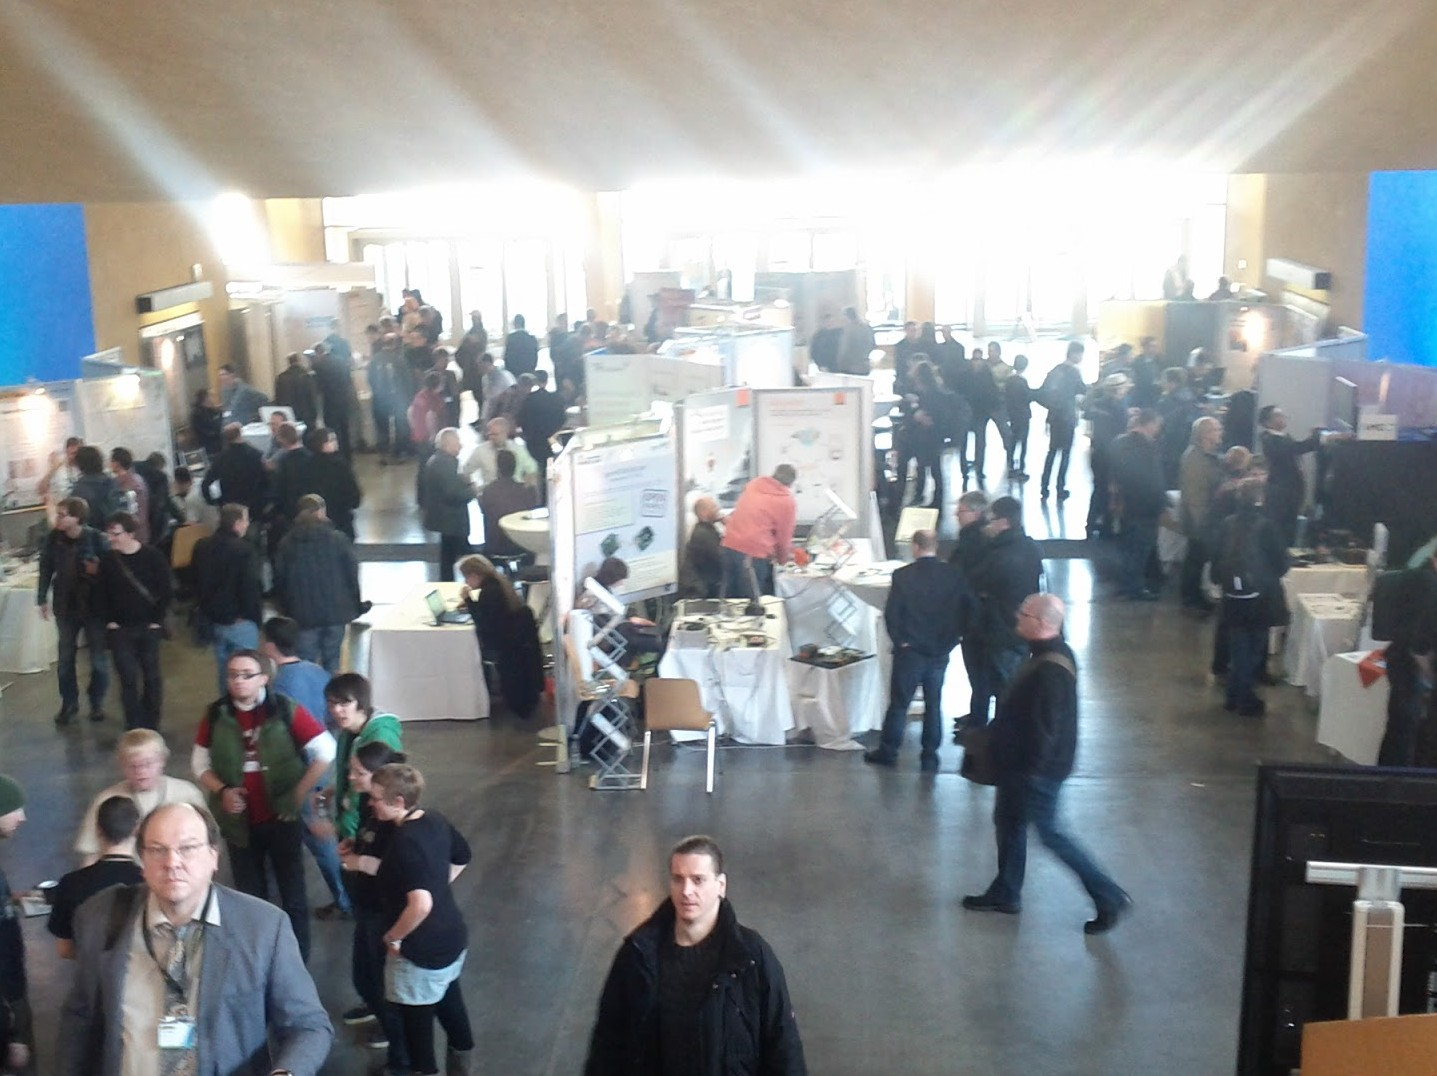
\includegraphics[width=\linewidth]{chemnitz/chemnitz_messe.jpg}
\footnotesize{Besucher am Chemnitzer Linuxtage 2013. Bildrechte: [1], cc-by-sa}
\end{center}

\subsection*{Linux in Schulen}

Der andere Vortrag den ich besucht habe war von \textbf{Kurt Gramlich} über den Einsatz (und das Scheitern) von \textbf{SkoleLinux} im deutschen Bundesland Rheinland-Pfalz. Kurt Gramlich ist ein sehr engagierter, weißhaariger Volkshochschul-Lehrer aus Nordreihn-Westfalen der sich über Jahre hinweg mit Linux in Schulen befasst hat. Als aus politischen Gründen das Bundesland Rheinland-Pfalz eine Microsoft-Alternative suchte und 'von oben' das Skolelinux-Projekt förderte war er stark darin involviert. Nachdem -aus politischen Gründen- das Bundesland Rheinland-Pfalz an Skolelinux nicht mehr interessiert war sprangen viele vorher beteiligte Schulen aus dem Projekt wieder ab.

Es gibt immer noch Schulen in Rheinland-Pfalz welche Skole-Linux verwenden, allerdings nicht mehr so viele wie zu Zeiten der offiziellen Projektförderung. Für mich waren vor allem folgende Erkenntnisse aus dem Vortrag interessant:

\begin{center}

\includegraphics[width=\linewidth]{chemnitz/chemnitz-kurt.jpg} \\
\footnotesize{Kurt Gramlich. Bildrechte: [3]}
\end{center}

\textit{Top-down vs. Bottom-Up}: Revolutionen (im Bildungsbereich) wirken nachhaltig von unten nach oben, nicht umgekehrt \\

\textit{Kulturelle Unterschiede}: Es gibt große kulturelle Unterschiede zwischen Skandinavien und Deutschland. In Skandinavien gibt es z.B. keine Schul-Internetfilter, in Deutschland werden sie von Behörden und Eltern verlangt. \\

\textit{Learning by Doing}: Die beste Art \textbf{SysAdmins} für ein SkoleLinuxSystem auszubilden ist es, engagierten Schülern so viel Verantwortung für die Schul-EDV wie möglich zu geben ('macht Euch das alles selbst aus'). Diese Schüler werden teils später erfolgreiche Admins. \\

\textit{Nehmen was da ist}: Die Schule sollte laut Kurt Gramlich nicht versuchen mit Gewalt Technologien zu unterrichten welche an der Lebenswirklichkeit der Schüler vorbeigehen sondern die Technologie benutzen welche die Schüler sowieso besitzen (Smartphones, Tablets) und versuchen damit etwas Vernünftiges zu machen. \\

\textit{Open Source braucht Zeit}: Linux / Open Source Neulingen sollte man als gutmeinender Open Source Evangelist nicht das Kostenargument (Linux kost' nix!) als \emph{den} Vorteil freier Software 'verkaufen'. Auch freie Software kostet: Zeit, Nerven und Support. Speziell für Schulen welche Raubkopien verwenden oder Ihre Software geschenkt / vom Staat bezahlt bekommen ist das Kostenargument zweitrangig. 

Der \emph{Geist von Open Source}, -das Erkennen und Erleben was freie Software bedeutet- dauert laut Kurt Gramlich 2 bis 3 Jahre, erst dann versteht ein neuer User dass er Teil einer Gemeinschaft ist, etwas geschenkt bekommt (Support, Bier, Schokolade...) und sich kreativ und hilfreich in diese Gemeinschaft einbringen kann. In einem Beratungsgespräch oder mit einer Gratis-CD ist diese Erfahrung nicht zu vermitteln.

%\begin{center}
%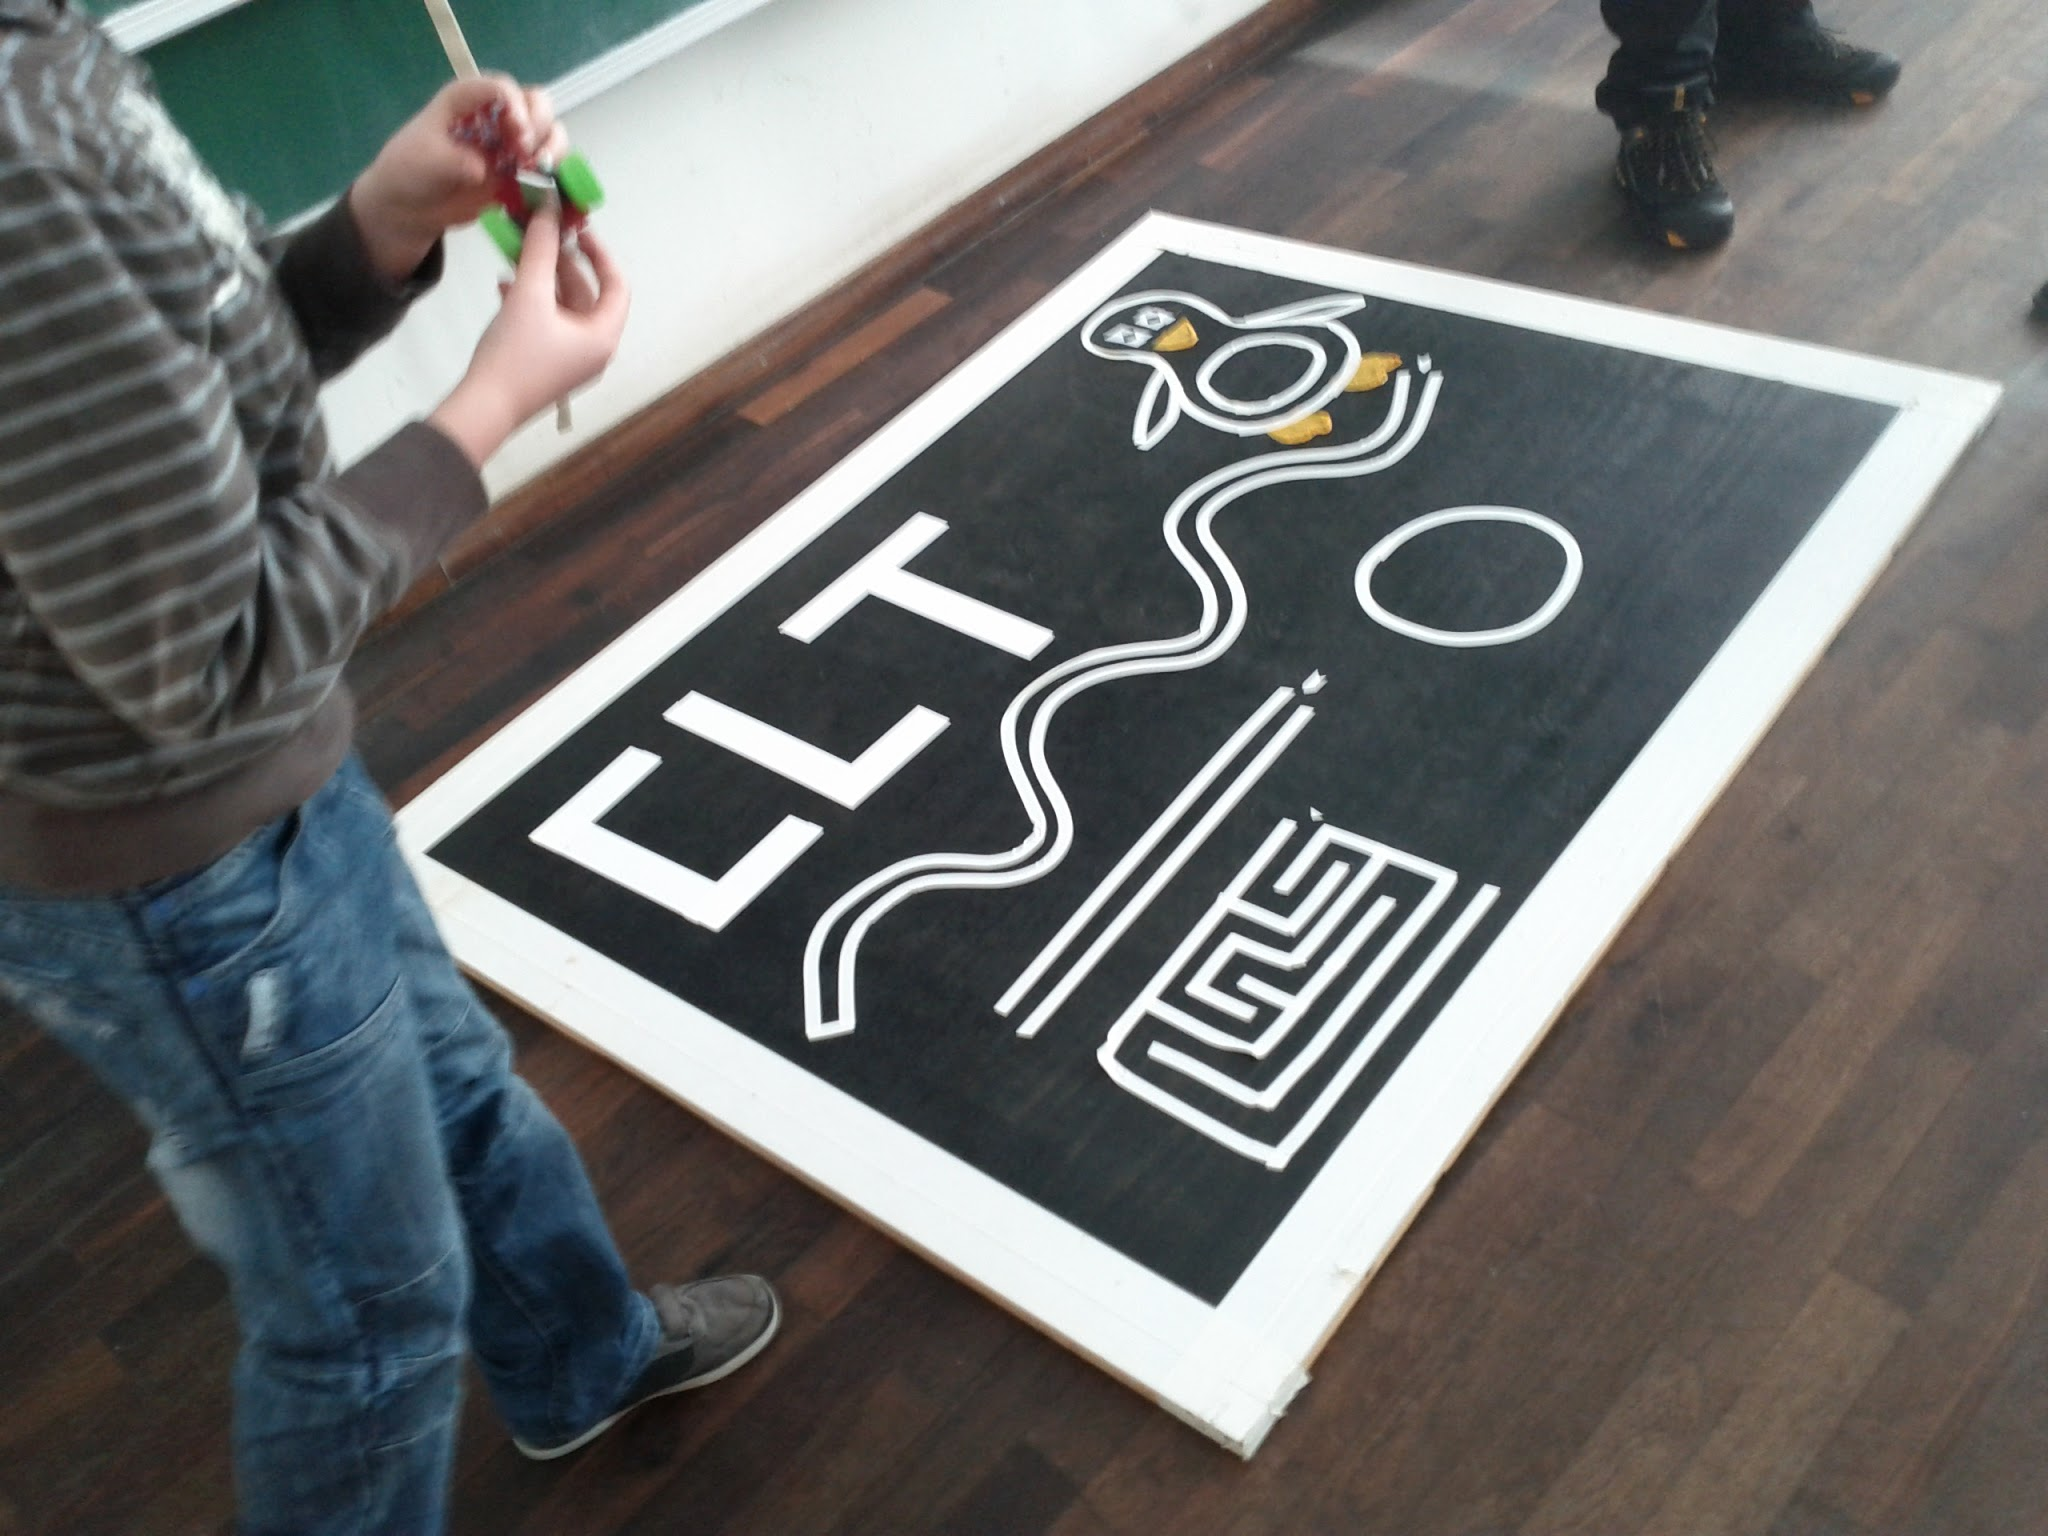
\includegraphics[width=\linewidth]{chemnitz/chemnitz_kinderzone1.jpg}
%\footnotesize{Chemnitzer Linuxtage 2013, Kinderzone. Bildrechte: [1], cc-by-sa}
%\end{center}

\subsection*{Go East!}
Neben der wirklich hervorragenden Organisation seitens der Chemnitzer Studierenden -es gab z.B. ein ständig gut gefülltes Buffet im Backstage Bereich für Standbetreuer- war ich angenehm überrascht von den Besuchern am \textbf{OSDomotics} Messestand. Viele Besucher hatten selber kleine Firmen oder waren Handwerker / Wohnungs- bzw. Haus-(um)bauer und hatten sofort Ideen was man mit einer Funkvernetzung von Sensoren und Aktoren machen könnte. Darunter waren Ideen (Gärtnereien, Alarmanlagen, Passivhäuser) auf welche wir OSDomotics Leute von selbst nicht gekommen wären. 

Außerdem erfuhr ich dass viele Firmen in Sachsen (\textbf{Silicon Saxony}) Mitarbeiter suchen - wegen dem Bevölkerungsrückgang und dem Abwandern vieler junger Studienabgänger nach Westdeutschland suchen die Firmen teils von Prag bis Portugal nach qualifizierten IT-Mitarbeitern und Facharbeitern.

\begin{center}

\includegraphics[width=0.5\linewidth]{chemnitz/chemnitz_logo14.png}
\footnotesize{Bildrechte: Chemnitzer Linuxtage 2014}
\end{center}

Ich freue mich schon auf den nächsten \href{http://chemnitzer.linux-tage.de/2014/en/info/}{Chemnitzer Linuxtag} (15. und 16. März 2014, siehe RIS Journal 001, \texttt{kalender}, Seite page \pageref{kalender}) und kann eine Reise dorthin jedem an Linux Interessiertem empfehlen.

\subsection*{Fachbegriffe:}
~~~\href{http://www.osdomotics.com/}{\textbf{OSDomotics}}: ist ein Verein der freie Software und freie Hardware im Bereich Haustechnik fördert. Der Verein entwickelt Sensoren (z.B. Temperaturfühler) und Steuerungen (z.B. eine Funksteckdose) welche drahtlos via \href{http://de.wikipedia.org/wiki/6LoWPAN}{\textbf{6LoWPAN}-Protokoll} miteinander kommunizieren. Damit ist es z.B. möglich per Android Smartphone vom Urlaub aus die Heizung im Haus einzuschalten oder die Feuchtigkeit zu überwachen.
\begin{center}

\includegraphics[width=\linewidth]{chemnitz/chemnitz_osd_domotics_logo-2881.png}
\footnotesize{Bildrechte: osdomotics.com}
\end{center}

\href{http://de.wikipedia.org/wiki/Hashtag}{\textbf{Hashtag}}: Durch Voranstellen einer Raute (\#, englisch: Hash) vor einen Begriff (englisch: Tag) kann dieser Begriff in Social Media Anwendungen leichter gefunden werden. \\

\href{http://de.wikipedia.org/wiki/6LoWPAN}{\textbf{6LoWPAN}} besonders energies-effizienter  Datenfunk-Standard für 'Das Internet der Dinge'\\

\href{http://geany.org/}{\textbf{Geany}} sehr beliebter freier (free/libre open Source) Texteditor für verschiedenste Programmiersprachen. Die \LaTeX Files für diese Zeitschrift werden z.B. mit Geany bearbeitet. \url{http://geany.org} \\

\href{https://www.djangoproject.com/}{\textbf{Django}}: Ein Web-Entwicklungs Framework. Ermöglicht die Programmierung komplexer Web-Projekte mit Datenbank-Anbindung (z.B. Webshops, Wikis etc) mit Hilfe der eleganten Programmiersprache \href{http://python.org}{Python}. \url{https://www.djangoproject.com} \\

\href{http://flattr.com}{\textbf{Flattr}}: \href{http://flattr.com}{\textit{flattr.com}} ist ein skandinavischer Spenden / Micropaying Dienst der vor allem in Europa bei der Podcast-Szene populär ist. \\

\href{http://de.wikipedia.org/wiki/Paretoprinzip}{\textbf{Paretoprinzip}}: oder die 80-20 Regel besagt dass oft 20 Prozent der Kunden/Pflanzen/Tätigkeiten 80 Prozent der Eträge bringen. \\

\href{http://www.skolelinux.org/}{\textbf{Skolelinux}} \href{http://skolelinux.org/}{skolelinux.org} ist ein aus Skandinavien kommendes Linux-Projekt welches auf den Einsatz in Schulen spezialisiert ist. Weitere Schul-Linuxe sind z.B. \href{http://www.edubuntu.org/}{\textit{Edubuntu [9]}}, \href{http://d4e.at/}{\textit{Desktop4Education [10]}}, \href{http://www.linuxadvanced.at/}{\textit{Linux Advanced [11]}} (beide aus Österreich) bzw. das Schweizer Projekt \href{http://www.imedias.ch/lernstick}{\textit{Lernstick [12]}}, welches gemeinsam mit Linux Advanced entwickelt wird. \\

%\begin{center}
%
\includegraphics[width=0.5\linewidth]{chemnitz_skole_tux_small.png}
%\footnotesize{Skolelinux Logo. Bildrechte: Skolelinux}
%\end{center}

\href{http://de.wikipedia.org/wiki/Systemadministrator}{\textbf{System-Administratoren, Sysadmins}} sind die technischen Betreuer eines großen, vernetzten Computersysteme.\\

\href{http://de.wikipedia.org/wiki/Silicon_Saxony}{\textbf{Silicon Saxony}}: eine Ansammlung von IT-Firmen aus den Bereichen Mikroelektronik und Photovoltaik, hauptsächlich im Raum Dresden, mit Ihren Zulieferern und dazugehörigen Firmen.

\subsection*{Podcast}
\begin{wrapfigure}{l}{2cm}
%\begin{center}

\includegraphics[width=2cm]{chemnitz/chemnitz-biertaucherlogo.png}
\end{wrapfigure}
%\end{center}
Einen ausführlichen Audio-Bericht von \href{http://spielend-programmieren.at}{Horst JENS} und Florian Schweikert über den Chemnitzer Linuxtage 2013  hören Sie im \href{http://spielend-programmieren.at/de:podcast:biertaucher:2013:096}{\textbf{Biertaucherpodcast 096}: \texttt{goo.gl/rmu79}}. 

\subsection*{Download, Feedback:}
\textbf{R.I.S.-Journal}, Ausgabe 001: \\
\href{http://spielend-programmieren.at/de:ris:001}{spielend-programmieren.at/de:ris:001}\\
\textbf{Download} Ordner, verschiedene Formate: \href{http://spielend-programmieren.at/risjournal/001/chemnitz}{\texttt{spielend-programmieren.at/\\risjournal/001/chemnitz}} \\
\textbf{Feedback} \Letter\ \texttt{horst.jens@spielend-\\programmieren.at} \\



\subsection*{Lizenz, Quellen:}
\begin{wrapfigure}{l}{2.0cm}

\includegraphics[width=2cm]{chemnitz/ccbysa88x31.png}
\end{wrapfigure}
Dieses Material steht unter der Creative-Commons-Lizenz Namensnennung - Weitergabe unter gleichen Bedingungen 4.0 International. Um eine Kopie dieser Lizenz zu sehen, besuchen Sie \url{http://creativecommons.org/licenses/by-sa/4.0/deed.de}. \\

\textbf{Quellen:} \\
{[}1{]} \href{http://spielend-programmieren.at}{spielend-programmieren.at} \\
{[}2{]} \href{http://chemnitzer.linux-tage.de/2013/}{chemnitzer.linux-tage.de/2013/} \\
{[}3{]} \href{http://wiki.skolelinux.de/KurtGramlich/Biografie}{http://goo.gl/Fa6mu2} \\
{[}4{]} \href{http://datenkanal.org/archives/14-Interview-mit-Kurt-Gramlich-zu-Skolelinux.html}{http://goo.gl/EoIDpy} \\
{[}5{]} \href{http://osdomotics.com}{osdomotics.com} \\
{[}6{]} \href{http://spielend-programmieren.at/de:sonstiges:alter_blog:2009:0318_chemnitzer_linux-tage_2009}{goo.gl/fUs552} \\
{[}7{]} \href{https://plus.google.com/u/0/112888349007751740309/about}{goo.gl/THuHS9} \\
{[}8{]} \href{http://biertaucher.at}{biertaucher.at} \\
{[}9{]} \href{http://www.edubuntu.org/}{edubuntu.org} \\
{[}10{]} \href{http://d4e.at/}{Desktop4Education} \\
{[}11{]} \href{http://www.linuxadvanced.at/}{linuxadvanced.at} \\
{[}12{]} \href{http://www.imedias.ch/lernstick}{imedias.ch/lernstick} 


